\chapter{Updatable Vector Tiles}\label{chapter_updatable_vector_tiles}


\osm{} contributors add more than three million nodes and ways every day.
In order to keep the prerendered tiles up to date this poses a challenge of looking at the changes
and figuring out which tiles are affected by those changes and schedule them for rerendering.

\begin{figure}[H]
  \centering
  \includegraphics[width=1.0\textwidth]{images/updatable_vectortiles_flow.png}
  \caption{Simplified diagram of changed tiles detection process}
\end{figure}

To find out which tiles are affected by updates requires a multi-step process.

\begin{enumerate}
    \item Find relevant \osm{} objects affected by the changes
    \item Calculate tiles covered by the object geometries
\end{enumerate}

\paragraph{Time Constraint} In order to be able to keep up with rendering changes the update process can not take longer than the number of days the database is behind.

\section{OSM Diff File}

\osm{} provides a single XML file, which contains every mapped object. Since the process of importing is time and resource consuming it is not feasible to redo this process to keep up with all the changes. Therefore OSM additionally provides hourly or daily diff files in the OsmChange format which contains the created, modified and deleted objects over a period of time. Importing only the subsequent diff files after an initial import allows to keep the database in sync with the latest changes.

\subsection*{Example}
The listing \autoref{create_modify_delete_xml} shows an example diff file which contains a create, modify and delete entry for different objects.

\begin{listing}[H]
  \centering
  \begin{xmlcode}
<?xml version='1.0' encoding='UTF-8'?>
<osmChange version="0.6" generator="Osmosis 0.43.1" timestamp="2016-05-20T11:32:32Z">
  <create>
    <node id="4196907493" version="1" uid="1" lat="46.9280366" lon="7.1163806">
      <tag k="amenity" v="pharmacy"/>
      <tag k="name" v="Amavita"/>
    </node>
  </create>
  <modify>
    <node id="4051684660" version="2" uid="1" lat="53.5705074" lon="9.9950888">
      <tag k="emergency" v="fire_hydrant"/>
      <tag k="ref" v="13874"/>
    </node>
    </modify>
  <delete>
    <node id="1044604768" version="2" uid="1" lat="52.6429848" lon="5.082264"/>
  </delete>
</osmChange>
  \end{xmlcode}
  \caption{Create, modify and delete example}
  \label{create_modify_delete_xml}
\end{listing}

\subsection{Different Change scenarios}\label{osm_change_scenarios}


\paragraph{Create object} A new object is created (e.g. a new point of interest is added). All tiles covered by the created object must be rerendered.

\paragraph{Delete object} An object gets deleted (e.g. an old house which does not exist anymore). All tiles covered by the deleted object must be rerendered.

\paragraph{Modify object} An object gets modified (e.g. add additional translations to a place). All tiles covered by the modified object must be rerendered.

\paragraph{Move object} An object is moved (e.g. an incorrectly mapped bus stop had to be repaired or has been moved in the real world). All tiles covered by the original object and all tiles covered by the moved object must be rerendered.

\section{Diff Import}

Imposm3 is used for the regular import of the OSM Planet file. Additionally it supports importing OSM Diff files. Imposm3 will read the XML File and calculate with the local cache of previous imports which nodes, ways and relations are affected by the changes.

If the changes would be mapped into the database existing entries in the database will first be removed using a SQL \texttt{DELETE} and then added again using SQL \texttt{INSERT}.\\\\

\begin{figure}[H]
  \centering
  \includegraphics[width=0.35\textwidth]{images/imposm3_operations_venn_diagram.png}
  \caption{Imposm3 SQL statements and OSMChange actions}
\end{figure}

The diff import functionality of imposm3 is only meant to keep the database in sync with the OSM changes. It is not possible to track which rows in the table have been inserted, updated or deleted. However this information is crucial to detect changed tiles and support all change scenarios from \autoref{osm_change_scenarios}.
The only way to keep track of changed features is to either modify Imposm3 or take actions at the database level.

\subsection{Track changes}

To track the entries at the database level the timestamp of the import is added to each object. This makes it possible to query modified and created objects by filtering for the latest import date.

To keep track of entries that are no longer present in the database (like deleted and moved objects) auditing of \texttt{DELETE} actions has been implemented.

\subsubsection{Track inserted rows}

The \texttt{timestamp} column is used to keep a history of inserted features. The \texttt{timestamp} column contains the date of the original PBF or OSC file the feature was defined or changed. This is important for calculating the changed tiles in a timeframe later on in \autoref{calculate-changed-tiles}.

\begin{enumerate}
   \item The imposm3 diff process inserts new rows for updated and added features
   \item The \texttt{timestamp} column is now set to \texttt{NULL} for all new rows
   \item Update the table and set the rows \texttt{timestamp} column to the timestamp of the import
\end{enumerate}

\subsubsection{Track deleted rows}

If \osm{} features are changed or removed imposm3 will first delete the row from the table and then insert it again (if it is an update). This is due to performance reasons since a \texttt{DELETE} followed by an \texttt{INSERT} is faster than an \texttt{UPDATE}.

To support the change scenarios of deleting, modifying and moving an object the \texttt{track\_osm\_delete} trigger is enabled for each table to keep track of deleted rows (similar to database auditing).

\begin{listing}[H]
  \centering
  \begin{sqlcode}
    DROP TRIGGER IF EXISTS osm_building_polygon_track_delete ON osm_building_polygon;
    CREATE TRIGGER osm_building_polygon_track_delete
    BEFORE DELETE ON osm_building_polygon
    FOR EACH ROW EXECUTE PROCEDURE track_osm_building_polygon_delete()
  \end{sqlcode}
  \caption{Delete trigger on a table}
\end{listing}

The trigger will track the deleted row in a separate audit table before discarding it.

\begin{listing}[H]
  \centering
  \begin{sqlcode}
CREATE OR REPLACE FUNCTION track_osm_building_polygon_delete() RETURNS TRIGGER AS $$
BEGIN
     IF (TG_OP = 'DELETE') THEN
        INSERT INTO osm_building_polygon_delete(id, geometry)
        VALUES($1, $2) USING OLD.id, OLD.geometry;
        RETURN OLD;
     END IF;
     RETURN NULL;
END;
$$ language plpgsql;

  \end{sqlcode}
  \caption{Logic of delete trigger}
\end{listing}

As a result each table has an additional delete tables which contains all deleted and modified rows. This allows in a second step to calculate the affected tiles and rerender them.

%----------------------------
\newpage{}
\section{Calculate changed tiles}\label{calculate-changed-tiles}

One way to determine which tiles are affected by changes in the database is to calculate the covered tiles from changed geometries by recursively descending the XYZ Quadtree and checking for intersections of the tiles and geometries.

\subsubsection*{Algorithm}

\begin{enumerate}  
    \item \label{itm:calc-extent}Calculate the extent $e$ for a given $(x,y,z)$ tile index
    \item \label{itm:bbox} Check if geometry $g$ intersects with the tile extent $e$ 
    \item Stop if there is no intersection in \ref{itm:bbox}
    \item Select tile index $(x,y,z)$
    \item Calculate the four child XYZ indizes \\
       \begin{pmatrix}
            x*2 & y*2 & z+1\\
            x*2+1 & y*2 & z+1\\
            x*2 & y*2+1 & z+1 \\ x*2+1 & y*2+1 & z+1
        \end{pmatrix}
    \item Call \ref{itm:calc-extent} for children if zoom level $z$ has not reached max zoom level $Z$
\end{enumerate}

\begin{figure}[H]
  \centering
  \includegraphics[width=0.9\textwidth]{images/polygon_xyz_matching.png}
  \caption{Recursive tile matching on polygon}
\end{figure}

\subsubsection*{Tile Buffers}

Geometries in vector tiles can extend beyond the boundaries of a tile (tile buffer).
To support the concept of a buffer in the algorithm the extent $e$ for the $(x,y,z)$ tile index
is extended by a custom buffer $b$. The tile usually has a resolution of $256$px. By adding the buffer to the tile $256 + 2 * b$ it is ensured that tiles that contain the geometries inside their buffers are detected as well.

\begin{figure}[H]
  \centering
  \includegraphics[width=0.7\textwidth]{images/polygon_buffer_xyz_matching.png}
  \caption{Recursive buffered tile matching on polygon}
\end{figure}


\subsubsection*{PostgreSQL Implementation}

The PostGIS implementation makes heavy use of the \texttt{\&\&} operator and GiST indizes on the geometry columns to check whether the tile extent and geometry intersect with each other. Although using the bounding box of the geometry is not accurate and can yield false positive changed tiles it is much faster than using the correct \texttt{ST\_Intersects}.

\begin{listing}[H]
  \centering
  \begin{sqlcode}
CREATE OR REPLACE FUNCTION overlapping_tiles(geom geometry, max_zoom_level INT, buffer_size INT)
RETURNS TABLE (tile_z INT, tile_x INT, tile_y INT) AS $$
BEGIN
    RETURN QUERY
        WITH RECURSIVE tiles(x, y, z, e) AS (
            SELECT 0, 0, 0, geom && XYZ_Extent(0, 0, 0, buffer_size)
            UNION ALL
            SELECT x*2 + xx, y*2 + yy, z+1,
                   geom && XYZ_Extent(x*2 + xx, y*2 + yy, z+1, buffer_size)
            FROM tiles, (VALUES (0, 0), (0, 1), (1, 1), (1, 0)) as c(xx, yy)
            WHERE e AND z < max_zoom_level
        )
        SELECT z, x, y FROM tiles WHERE e;
END;
$$ LANGUAGE plpgsql IMMUTABLE;
  \end{sqlcode}
  \caption{Recursive tile matching of geometry}
\end{listing}


\subsection{Point Optimization}

Points always fit into a single tile at each zoom level.
Therefore given a point the covered tile can immediately be calculated. The recursive descend algorithm is not needed for this.

\begin{figure}[H]
  \centering
  \includegraphics[width=0.9\textwidth]{images/point_xyz_matching.png}
  \caption{Tiles covering a point geometry}
\end{figure}


\begin{listing}[H]
  \centering
  \begin{ccode}
#include "math.h"
float8 D2R = M_PI / 180.0;

// Latitude and longitude of Zurich
int32 zoom_level = 14;
float8 lat = 47.376887;
float8 lon = 8.541694;

float8 _sin = sin(lat * D2R);
float8 z2 = pow(2, zoom_level);

// XYZ Tile index calculated from latitude and longitude
int32 x = floor(z2 * (lon / 360 + 0.5));
int32 y = floor(z2 * (0.5 - 0.25 * log((1 + _sin) / (1 - _sin)) / M_PI));

  \end{ccode}
  \caption{Calculate tile at given zoom level for a point}
\end{listing}

\subsection{Export changed tiles}

The algorithm defined in \autoref{calculate-changed-tiles} is applied over all geometries that have changed since a given timestamp to find out all unique tiles that are affected by the changes and need to be rendered again.

\begin{listing}[H]
  \centering
  \begin{sqlcode}
    SELECT DISTINCT t.tile_x AS x, t.tile_y AS y, t.tile_z AS z
    FROM osm_building_polygon AS g
    INNER JOIN LATERAL overlapping_tiles(g.geometry, 14, 4) AS t
    ON g.timestamp >= (LOCALTIMESTAMP - INTERVAL '7 days')
  \end{sqlcode}
  \caption{Calculate all tiles containing building polygons that changed in the last 7 days}
\end{listing}

\begin{figure}[H]
  \centering
  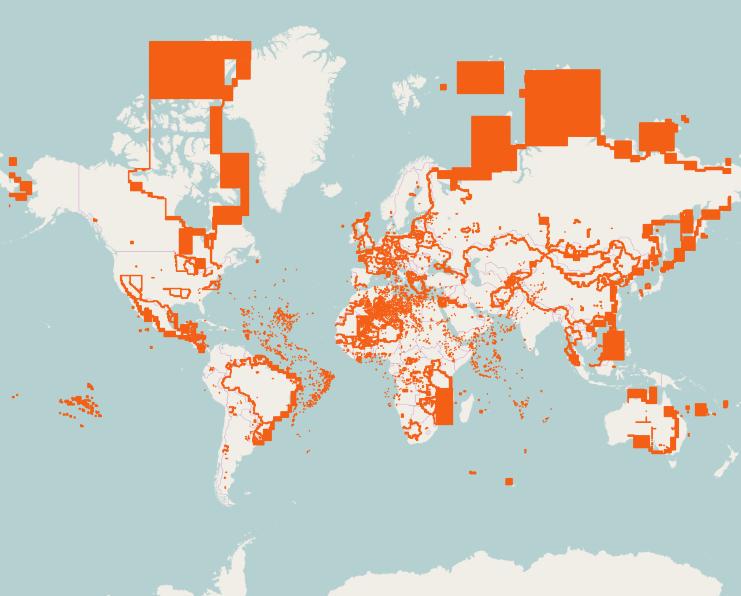
\includegraphics[width=1\textwidth]{images/changed_tiles_z10.png}
  \caption{Changed tiles on z10 over course of 10 days}
\end{figure}
